%!TEX root = ../../thesis.tex

\graphicspath{{Chapters/appendix_bonsai/figures/}}

\section{Choosing lambda graphs}
We can visualize these pruning patterns by encoding each edge's operation choice as a binary vector of size
$|\mathcal{O}|$, where a 0 at the $i$th digit of the vector represents that the $i$th operation has been hard-pruned from
the edge. For our example models, this is a binary vector of size 7, meaning there are 128 unique edge combinations.
We can represent the particular combination of operations within an edge as an integer between 0 and 127, with
$0=[0,0,0,0,0,0,0]$ representing all operations pruned, while $127=[1,1,1,1,1,1,1]$ represents all operations preserved.
Using a parallel coordinate plot we can use these encodings to visualize how each edge in a model evolves over the
training lifetime, showing both the pruning patterns the edge gravitate to as well as the speed which they arrive at those
patterns. Figure~\ref{fig:lambdapcps} shows these parallel coordinate plots for all three test models, and shows that our
intuition was correct. The first two models prune slowly and methodically, while the third prunes very rapidly and significantly.
Notably, the $\lambda=1.000$ soft-compresses to $0.5$ within the first few batches of training, and hard compresses to
that mark as soon as the first deadheading pass occurs. While these plots obfuscate the true proximity of edge configurations due to being a seven dimensional projection
into a single axis, they are useful to show that all of these decisions are decidedly non-random. For comparison,
Figure~\ref{fig:true_random} shows a completely random compression policy.

\begin{figure}[ht]
    \centering
	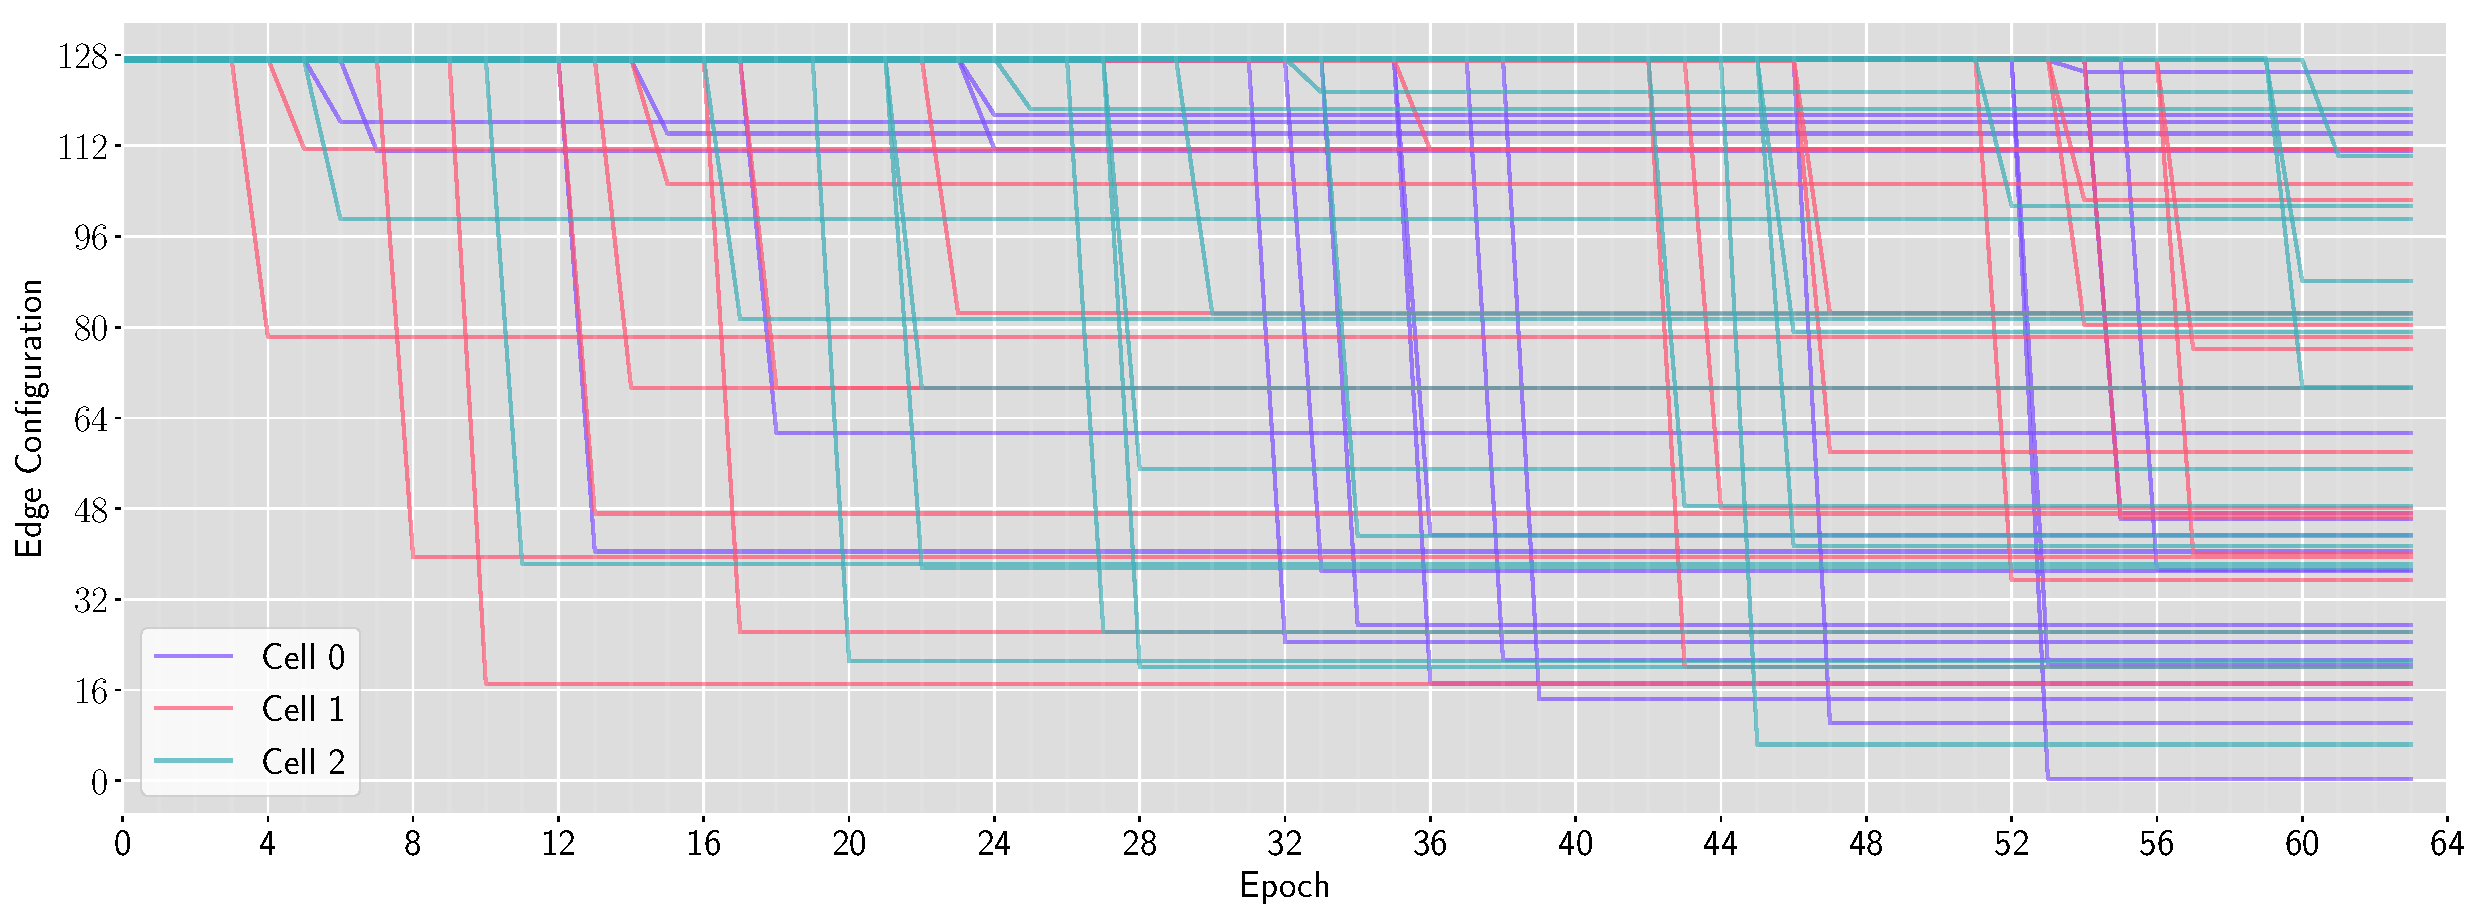
\includegraphics[width=\textwidth]{lambda_exps/true_random}
	\caption{True random compression: edges select a random state at a random epoch between 4 and 64. Notice the
	lack of clustering or power-2 gaps.}
	\label{fig:true_random}
\end{figure}


\begin{figure}
    \subfloat[Pruning patterns for $\lambda = 0$. In this freely motivated compression run, compression (marked by the state transitions) happens throughout training,
	as the model adapts to its needs at different stages of lifetime. .]{\label{fig:lambda0}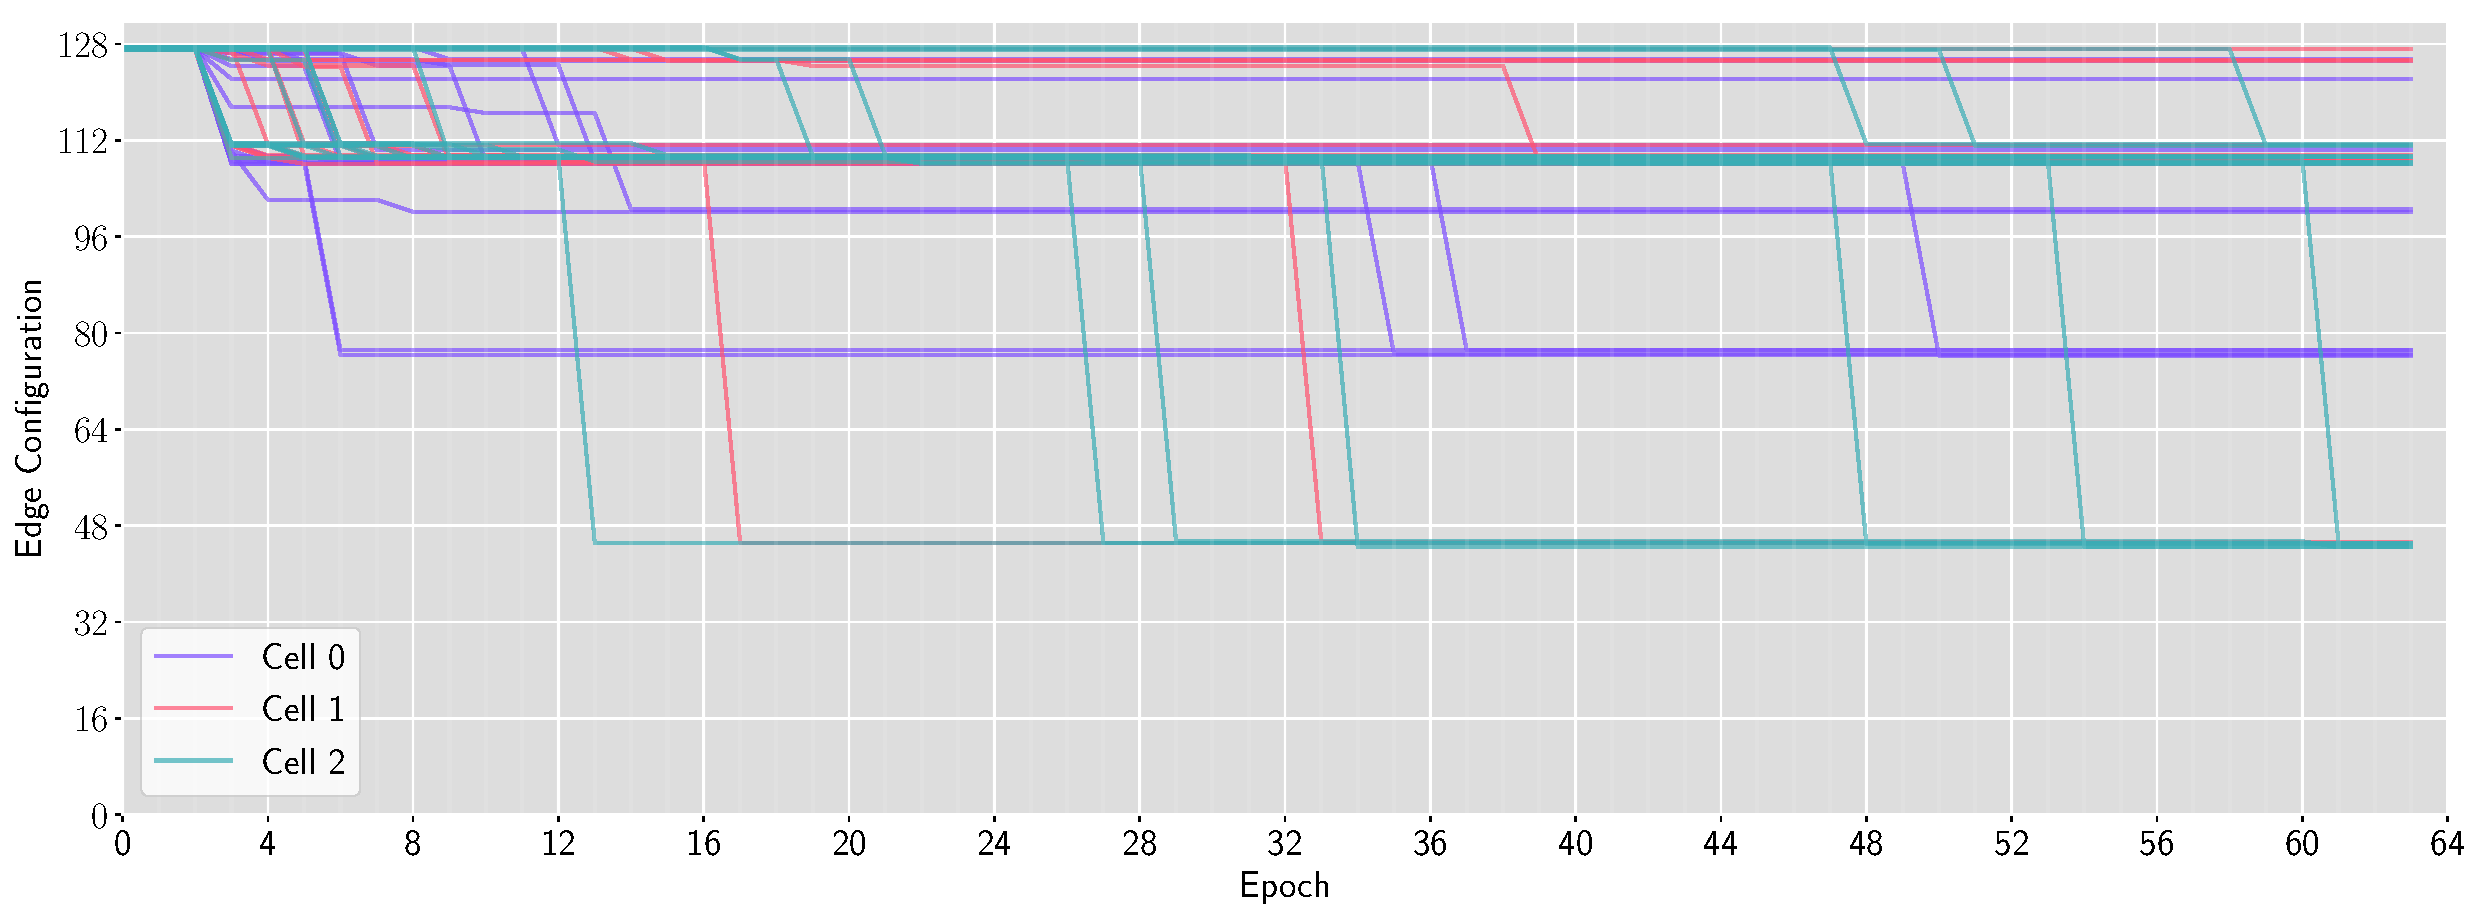
\includegraphics[width=\textwidth]{lambda_exps/lambda0_op_configurations}} \\
    \subfloat[Pruning patterns for $\lambda = 0.1$. Again, compression happens throughout the model lifespan.]{\label{fig:lambda01}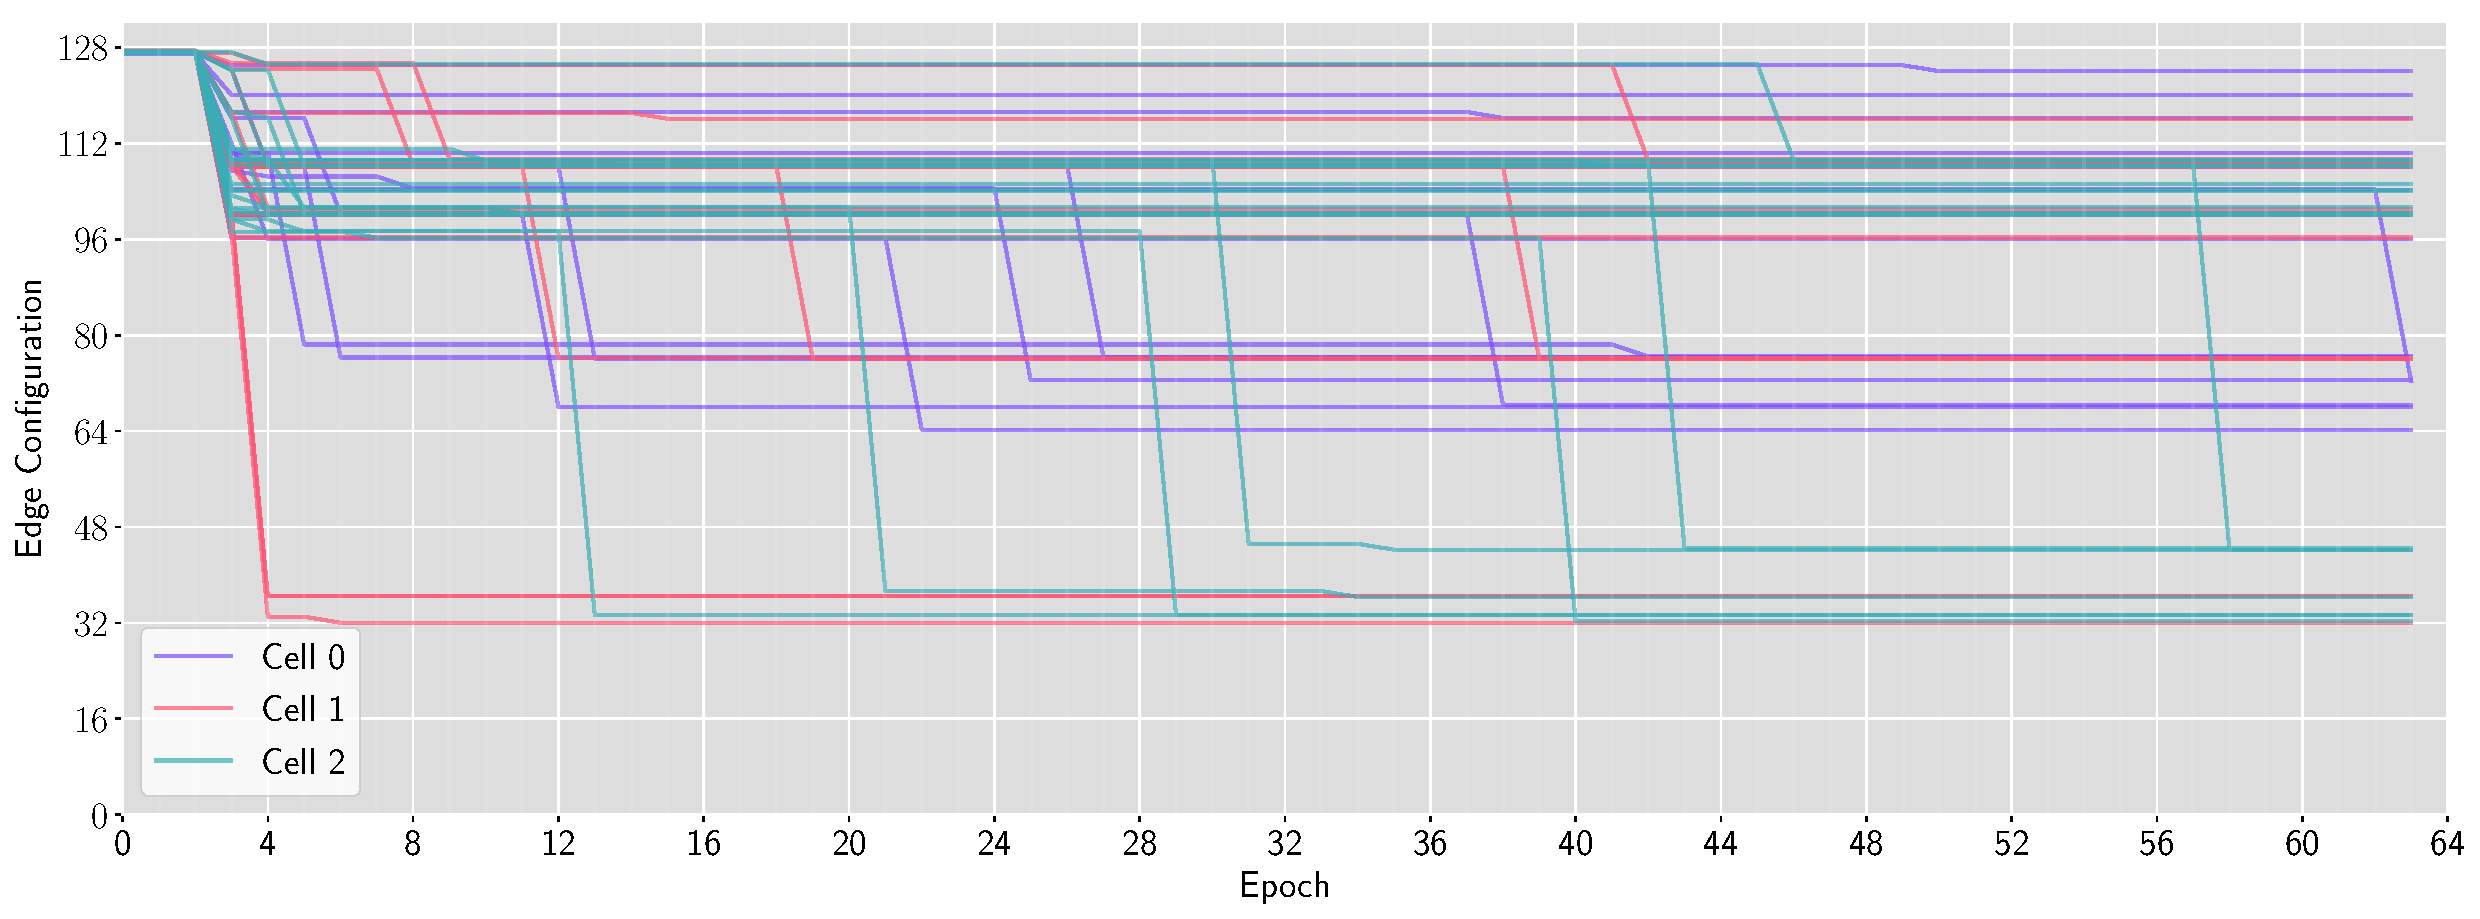
\includegraphics[width=\textwidth]{lambda_exps/lambda01_op_configurations}} \\
	\subfloat[Pruning patterns for $\lambda = 1000$. The model makes a significant amount of its pruning decisions within the first 9 epochs, with only 7 changes made afterward and none after the halfway point.]{\label{fig:lambda10}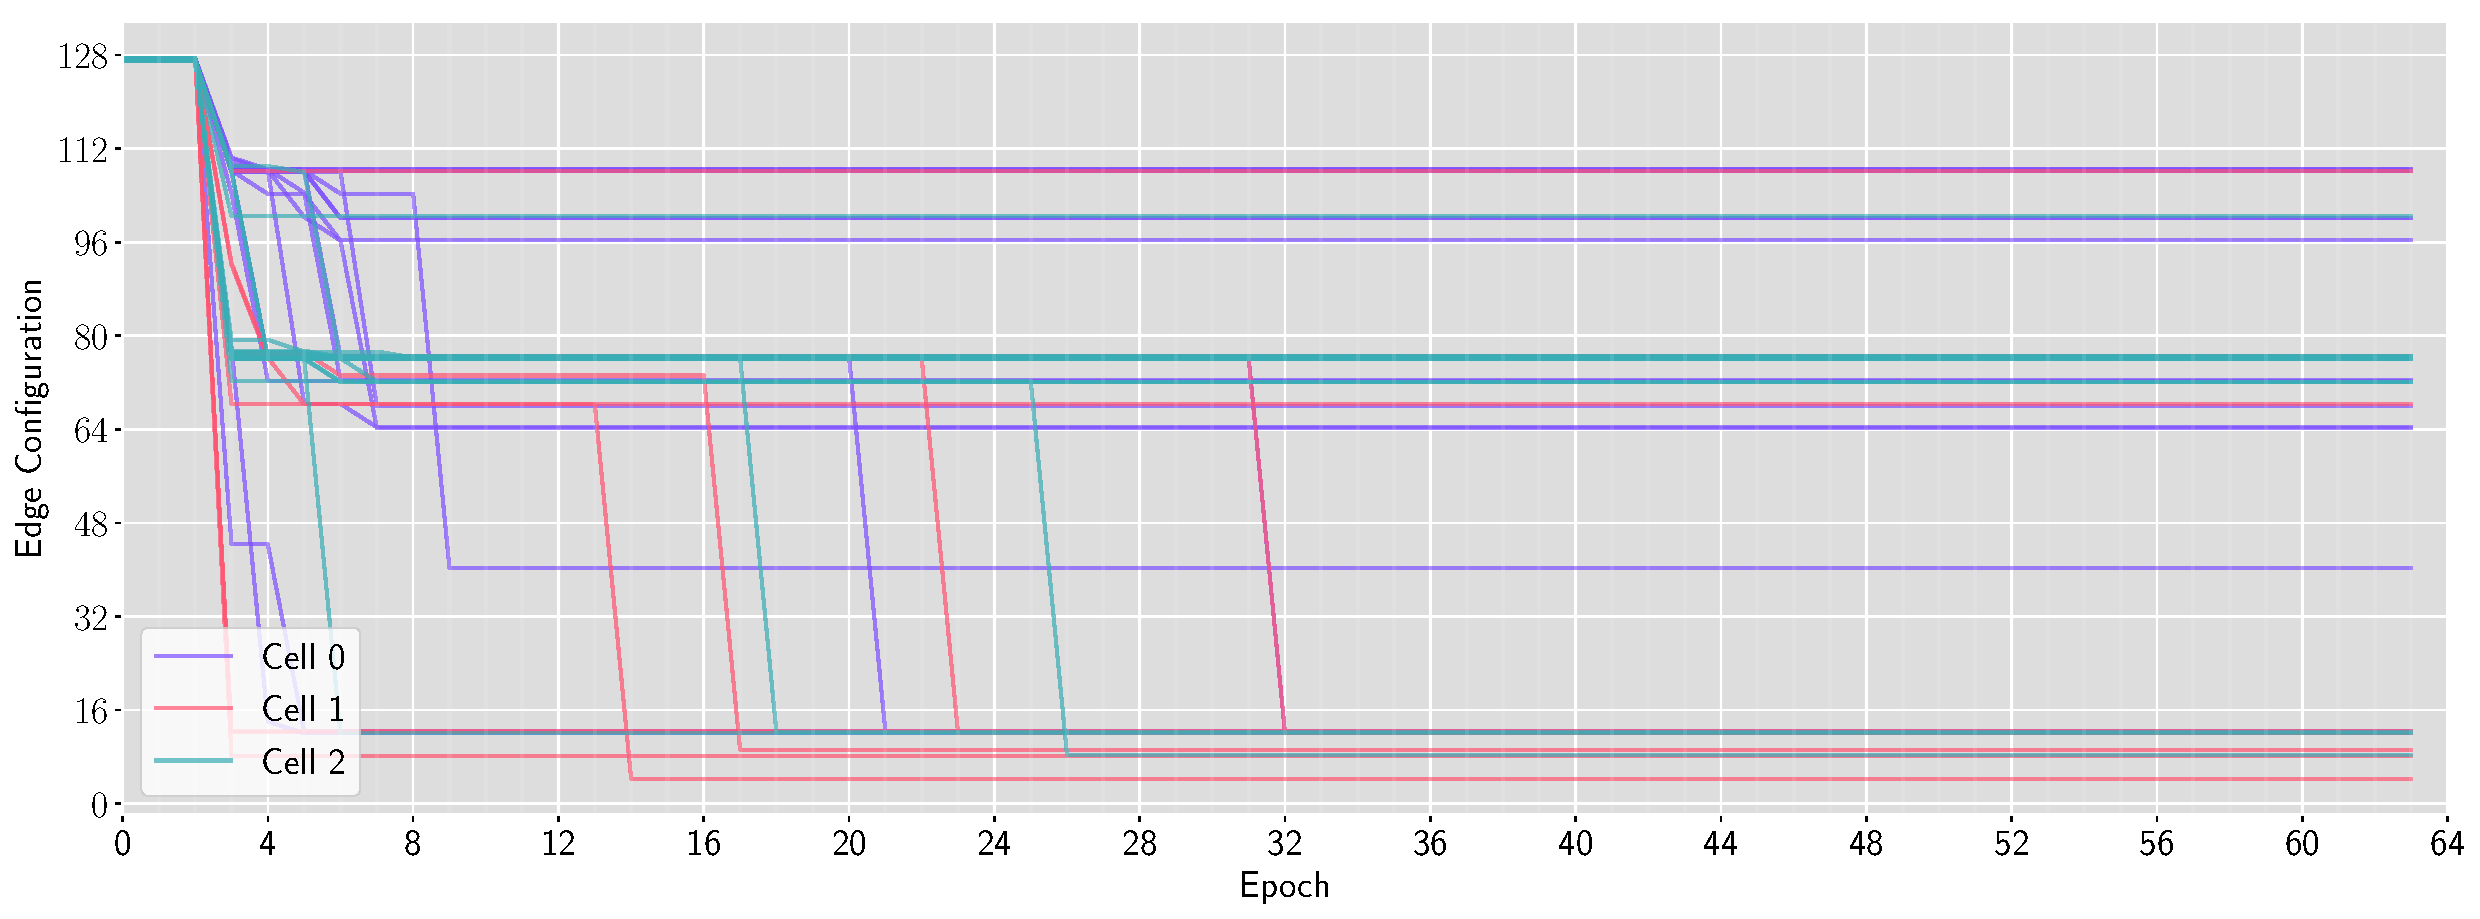
\includegraphics[width=\textwidth]{lambda_exps/lambda1000_op_configurations}}
	\caption{Parallel coordinate plots of model edge configuration over the course of training. Notice that in addition to
	clustered configurations, each plot has repeating, consistently shaped gaps of empty space. The sizes of these gaps
	correspond to powers of 2, and are indicative of higher-dimensional clustering obfuscated by this projection.}
	\label{fig:lambdapcps}
\end{figure}
\newpage


\ndspzbd

 Originally, the size of operations was measured in isolation. First, the current Torch memory allocation
was measured. Next, the desired operation and pruner was initialized, and data of the specified shape was passed through.
This process was repeated some $n$ times, after which the Torch memory allocation was sampled again. The size of the operation
was taken as the difference in allocations divided by $n$. This algorithm is described in more detail in
Algorithm~\ref{alg:original_operation_sizing}.

\begin{algorithm}
	\SetAlgoLined
	let $\mathcal{M}$ refer to measuring the current Torch memory allocation\;
	$m_{pre} = \mathcal{M}$\;
	\For{$0 \to n$} {
		Initialize operation $o$ and pruner $p$\;
		Pass sample input of specified shape \textit{forwards} through $o$ and $p$\;
	}
	$m_{post} = \mathcal{M}$\;
	\KwResult{$\frac{m_{post}-m_{pre}}{n}$}
	\caption{Original Operation Sizing}
	\label{alg:original_operation_sizing}
\end{algorithm}

However, this algorithm suffers from four design flaws that negatively affect the accuracy of its size estimation.
First, it does not take into account the backwards allocation of each operation. When Torch backpropagates the
gradients backwards through the computational graph, it must allocate gradient tensors at certain steps along the way. This
can increase the size requirements for an operation, by an amount that is not necessarily correlated with the forwards
size of the operation. Next, each initialized operation only ever sees a single sample input. This produces
inaccurate measurements due to a weird quirk in Torch VRAM allocation: the first forwards/backwards pass allocates a
certain amount of memory, but the second pass expands that allocation marginally. The allocation for the model remains
fixed from the second batch onwards, meaning that we need to ``warmup'' the operation with at least two batches for an accurate measurement.
My hunch is that this slight extra allocation comes from operations that contain things like batch normalizations which track running means across batches,
and thus require tensor space to store something like current and previous batch statistics. The third design flaw comes
from only measuring memory allocation at the beginning and end of the simulation, which only accurately reflects the memory
requirements if the allocation is monotonically increasing throughout the calculation process. However, in practice Torch allocates and deallocate memory
throughout the simulation process, which changes the memory delta depending on when you measure it. Finally, this
simulation only measures the operations independently, without considering how interaction effects between operations might affect
memory allocation.

\begin{algorithm}
	\SetAlgoLined
	let $\mathcal{M}$ refer to measuring the current Torch memory allocation\;
	$m = 0$\;
	\For{$0 \to n$} {
		$\mathbf{m} = \varnothing$\;
		$m_{pre} = \mathcal{M}$\;
		Initialize operation $o$ and pruner $p$\;
		\For{$0 \to n$} {
			$\mathbf{m} = \mathbf{m} \bigcup (\mathcal{M} - m_{pre})$\;
			Pass sample input of specified shape \textit{forwards} through $o$ and $p$, store output\;
			$\mathbf{m} = \mathbf{m} \bigcup (\mathcal{M} - m_{pre})$\;
			Add output to itself\;
			$\mathbf{m} = \mathbf{m} \bigcup (\mathcal{M} - m_{pre})$\;
			Pass output through sample loss function\;
			$\mathbf{m} = \mathbf{m} \bigcup (\mathcal{M} - m_{pre})$\;
			Pass gradient \textit{backwards} through $o$ and $p$\;
		}
		$m = m + \max(\mathbf{m})$
	}
	\KwResult{$\frac{m}{n}$}
	\caption{Compensated Operation Sizing}
	\label{alg:revised_operation_sizing}
\end{algorithm}

Fixing the backwards allocation issue is simple, just include a backwards pass of the gradients through the operation
within the simulation. The warmup issue is similarly straightforward to fix, simply by
repeating the forwards and backwards passes a number of times. To account for the non-monotonic allocation, the memory
allocation delta is recorded after each step of the simulation, and the maximum delta throughout an operation's lifespan
is recorded as its memory allocation. This is of course the relevant value here; regardless of the final allocation size
of an operation, its maximum size determines whether or not we face an out-of-memory error. Finally, we can take into account
operational interaction effects on their size by considering how the relevant interaction effects occur. Namely, as each
operation arrives in a node, in must be summed together with the other inbound operations. Therefore, each operation
after the first incurs a summation operation, which results in a tensor allocation. That means that in the most
common case (where an operation is not the first operation to arrive at a node) this extra summation and therefore
tensor allocation occurs,
which we can model in the simulation by adding the output of the operation to itself. Algorithm~\ref{alg:revised_operation_sizing}
shows the revised sizing estimation process, the accuracy of which will be evaluated shortly.

With a hopefully accurate operation size estimate, we design a method of packing our simulation model
$M'$ to the target compression level. To do this, the problem is approached one cell at a time, with each cell allocated
operations independently of one another. For each cell $C$ and for each operation dimensionality $d$ with that cell,
the set of operations $\mathcal{O}_{C,d}$ within is collected. This means the total size of that set of operations can be easily
estimated as the sum of the estimated size of each operation:
\newcommand{\size}{\text{size}}
\begin{align}
	\size(\mathcal{O}_{C,d}) = \sum_{o \in \mathcal{O}_{C,d}}{\size(o)} \label{eq:additive sizing}
\end{align}
The total size of the cell is therefore:
\begin{align}
	\size(C) = \sum_{d \in C} \; \sum_{o \in \mathcal{O}_{C,d}}{\size(o)}
\end{align}
To find the allocational size of the cell that gives the desired compression, the cell size is multiplied by
$c_{tgt}$. By the distributive property:
\begin{align}
	s_{tgt} = c_{tgt} * \sum_{d \in C} \; \sum_{o \in \mathcal{O}_{C,d}}{\size(o)} \\
	s_{tgt} = \sum_{d \in C} \; c_{tgt} \sum_{o \in \mathcal{O}_{C,d}}{\size(o)}
\end{align}
This means that the allocational problem can be reduced to finding the set of operations
$\mathcal{O}' \subset \mathcal{O}_{C,d}$ such that $\size(\mathcal{O}')=c_{tgt} * \size(\mathcal{O}_{C,d})$ for all
$C, d$ within the model. This can be accomplished by using a greedy change-making algorithm, that selects operations for
the chosen subset according to some heuristic over the available operations. In the process of designing this algorithm
three different heuristics have been used at various times: maximum, random, and minimum selection.
All three heuristics create a set of available operations $\mathcal{O}_{avail}$, which contains all unselected operations
that can be added to $\mathcal{O}'$ without increasing its total size above the target. The maximum heuristic then selects
the largest operation within $\mathcal{O}_{avail}$ to be added to $\mathcal{O}'$, the minimum selects the smallest, and
the random selects an operation at random. The selected operation is added to $\mathcal{O}'$, and the algorithm repeats.
Once there are no more operations that are eligible for $\mathcal{O}_{avail}$, the $\mathcal{O}'$ is fully allocated and the
algorithm ends. This process is detailed in full in Algorithm~\ref{alg:operation packing}.

\begin{algorithm}
	\SetAlgoLined
	let $\mathcal{O}_{M'} = \varnothing$\;
	\For{\upshape cell $C \in M'$} {
		\For{\upshape operation dimension $d \in \; C$} {
			let $\mathcal{O}_{C,d}$ equal the set of all operations in $c$ with dimension $d$\;
			let $\mathcal{O}' = \varnothing$ \;
			let $s_{tgt} = c_{tgt} \left( \sum_{o \in \mathcal{O}_{C,d}}{\size(o)} \right) $\;
			\While{$s_{current} < s_{aim}$} {
				let $s_{min} = \min_{o \in \mathcal{O}_d} \size(o)$\;
				\eIf{$s_{min}+s_{current} > s_{tgt}$ or $\mathcal{O}_{C,d} \setminus \mathcal{O}'=\varnothing$}{
					break;
				}{
					let $\mathcal{O}_{avail} = \{ o | o \in \mathcal{O}_{C,d} \setminus \mathcal{O}', \quad \size(\mathcal{O}') + \size(o) \le s_{tgt} \}$\;
					Choose $o_{chosen}$ from $\mathcal{O}_{avail}$ according to some heuristic $H(\mathcal{O}_{avail})$\;
					$\mathcal{O}' = \mathcal{O}' \cup \{o_{chosen}\}$\;
					$\mathcal{O}_{C,d} = \mathcal{O}_{C,d} - \{o_{chosen}\}$\;
				}
			}
			$\mathcal{O}_{M'} = \mathcal{O}_{M'} \cup \mathcal{O}'$\;
		}
	}
	\caption{Operation Allocation}
	\label{alg:operation packing}
\end{algorithm}

The rationale for evaluating different heuristics of operation selection stems from the original inaccurate operation
sizing algorithm. The four inaccuracies of estimation meant that while operation sizing and thus compression were generally
correlated with model size, it was not the nice linearly additive correlation expected by equation~\ref{eq:additive sizing}.
This meant that models allocated to a certain compression $c_{tgt}$ by the different heuristics would have different VRAM sizes despite
identical compression values. Since the entire reason for evaluating the size of these simulation models is to evaluate
whether a certain compression level fits into memory, I was forced to find the largest model at any compression
target. In the very first implementation, I chose the maximum heuristic as it is the most common choice for a greedy
change making algorithm. However, the inaccuracy of the original sizing was proportional to the number of the operations
in the model; models with fewer operations were smaller in VRAM size than those with more, despite both having identical
compression levels. The max heuristic recovers a solution that packs models with roughly the fewest operations possible,
which means that with the inaccurate original sizing metric these models were the smallest models of that particular
compression. To remedy this, I tried the minimum heuristic to fill models with the most number of operations possible.
However, the minimum heuristic produces suboptimal packing, and tends to be unable to produce models that are close
to the target compression. As such these models were literally smaller than might be expected, and did not serve as
representative $M'$ for the simulations. To avoid both issues, I used the random heuristic, which produces a solution
somewhere in the middle. Since it is able to pick large operations early, it can avoid the subpar packing of the minimum
heuristic, while still picking enough small operations to ensure that the model is closer to the largest model at that
compression.

However, this is all merely treating the symptoms, not the cause of the issue. If we can produce an operation sizing
that is accurate enough to recover the desired linear additivity, the number of operations in the model should have
no bearing on the compression. Using our revised operation sizing algorithm, we can evaluate its accuracy by comparing
the correlations between compression, operation counts, and model size, which are shown in Figure~\ref{fig:changemaking}.

\begin{figure}[ht!]
    \centering
	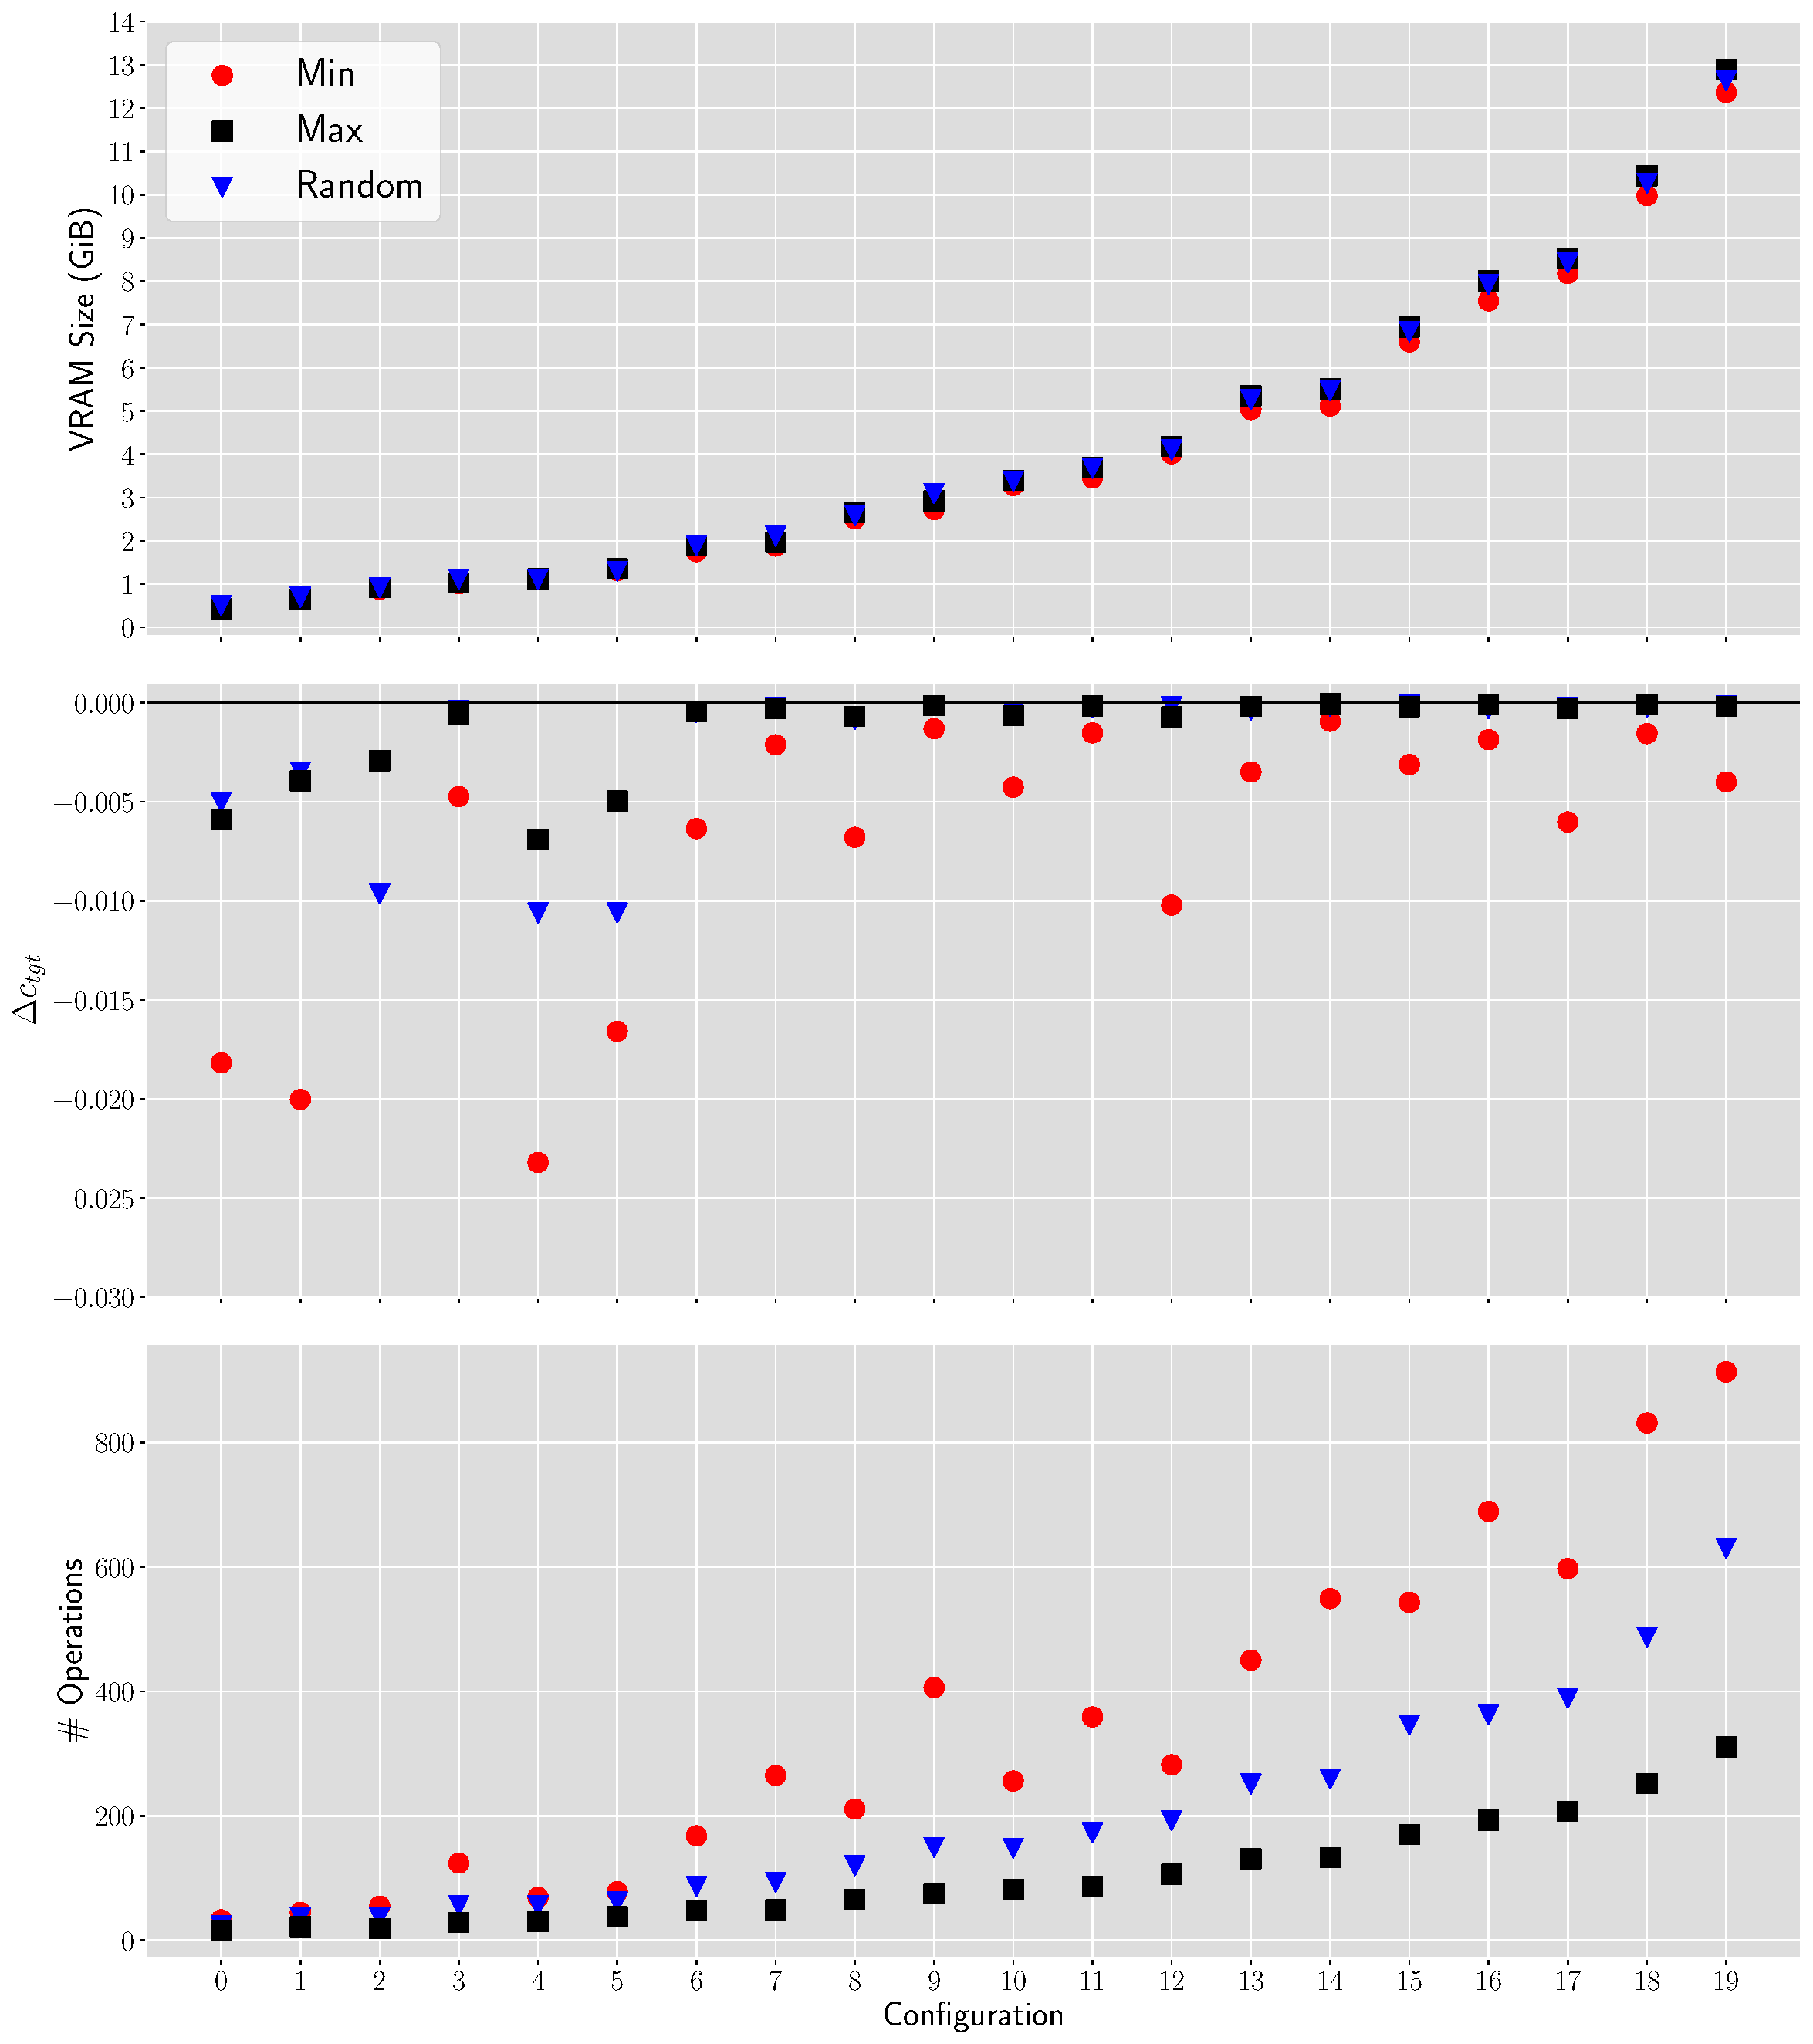
\includegraphics[width=\linewidth]{binpacking} \\
	\caption{Comparison of three different operation selection heuristics within the greedy-change making algorithm.
	60 models were allocated in total, corresponding to 20 different configurations each allocated operations by three
	heuristics.	Shown are the VRAM size (top),  difference between target compression
	and allocated compression (middle), and number of operations (bottom) plotted against configuration and heuristic.}
	\label{fig:changemaking}
\end{figure}

Here I pack 20 different model configurations according to the three heuristics and measure the resulting model's
VRAM size, delta to compression target, and operation count. To measure the VRAM size of any particular model, I first take
note of the VRAM allocation prior to the model's initialization. I then move the model onto the GPU and note the
VRAM allocation after passing tw full data batches through the model both forwards and backwards.
Two batches are necessary for accurate size measurement due to the same allocational ``warmup'' condition as described earlier.
To avoid potential stuck-tensor issues if the simulation model encounters an Out-of-Memory error, simulation models
 are initialized in a subprocess forked from the main process. This means there is a separate Torch context initialized in
the subprocess, which means that all tensors initialized in the subprocess are compartmentalized from those in the
main process. If the subprocess simulation model encounters an Out-of-Memory error, the process returns a failing exit
code and terminates. When the subprocess terminates, its Torch context deletes and garbage collects all tensors
that were initialized within it, cleaning any potentially orphaned tensors off of the GPU.
Essentially, the subprocess sandboxes the simulations from the main process, meaning we can size test without
worrying about destroying the viability of our main process.

Notice that the three heuristics do indeed
produce models that are consistently ranked in terms of operation count; the maximum heuristic chooses the fewest operations,
followed by random, and minimum chooses the most. Despite this, the VRAM size of the models are highly consistent despite
the operation count disparities, meaning that maximum heuristic is choosing a few large operations, while the minimum is
choosing many small operations. Additionally, we notice the same suboptimal packing behavior from the
minimum heuristic, which means those models undershoot the compression target and are thus smaller than the models
produce by the other two metrics. Overall, the sizing demonstrates the exact behavior that we hoped for,
that compression has become roughly injective with VRAM size, independent from operation count.

This is tremendously useful for our use-case because we have no way of providing any guarantee about a model's
real-world connectivity and operation count as it prunes to a certain compression level. It might prefer a small or large
operation count, meaning that the way that is achieves that specific compression is highly dependent on its individual
circumstances. If the relation between VRAM size and compression is dependent on operation count, we are forced to use the
worst-case, highest operation count model to determine whether a certain model compression fits into the VRAM size. This
means that any model that organically reaches that compression level at a lower operation count will actually be smaller
than necessary, and thus overpruned to its possible detriment. With the accurate sizing, we can instead be sure that any
model at a particular compression will fit if the simulation model does.